% Options for packages loaded elsewhere
\PassOptionsToPackage{unicode}{hyperref}
\PassOptionsToPackage{hyphens}{url}
%
\documentclass[
]{article}
\usepackage{amsmath,amssymb}
\usepackage{iftex}
\ifPDFTeX
  \usepackage[T1]{fontenc}
  \usepackage[utf8]{inputenc}
  \usepackage{textcomp} % provide euro and other symbols
\else % if luatex or xetex
  \usepackage{unicode-math} % this also loads fontspec
  \defaultfontfeatures{Scale=MatchLowercase}
  \defaultfontfeatures[\rmfamily]{Ligatures=TeX,Scale=1}
\fi
\usepackage{lmodern}
\ifPDFTeX\else
  % xetex/luatex font selection
\fi
% Use upquote if available, for straight quotes in verbatim environments
\IfFileExists{upquote.sty}{\usepackage{upquote}}{}
\IfFileExists{microtype.sty}{% use microtype if available
  \usepackage[]{microtype}
  \UseMicrotypeSet[protrusion]{basicmath} % disable protrusion for tt fonts
}{}
\makeatletter
\@ifundefined{KOMAClassName}{% if non-KOMA class
  \IfFileExists{parskip.sty}{%
    \usepackage{parskip}
  }{% else
    \setlength{\parindent}{0pt}
    \setlength{\parskip}{6pt plus 2pt minus 1pt}}
}{% if KOMA class
  \KOMAoptions{parskip=half}}
\makeatother
\usepackage{xcolor}
\usepackage[margin=1in]{geometry}
\usepackage{graphicx}
\makeatletter
\def\maxwidth{\ifdim\Gin@nat@width>\linewidth\linewidth\else\Gin@nat@width\fi}
\def\maxheight{\ifdim\Gin@nat@height>\textheight\textheight\else\Gin@nat@height\fi}
\makeatother
% Scale images if necessary, so that they will not overflow the page
% margins by default, and it is still possible to overwrite the defaults
% using explicit options in \includegraphics[width, height, ...]{}
\setkeys{Gin}{width=\maxwidth,height=\maxheight,keepaspectratio}
% Set default figure placement to htbp
\makeatletter
\def\fps@figure{htbp}
\makeatother
\setlength{\emergencystretch}{3em} % prevent overfull lines
\providecommand{\tightlist}{%
  \setlength{\itemsep}{0pt}\setlength{\parskip}{0pt}}
\setcounter{secnumdepth}{-\maxdimen} % remove section numbering
\ifLuaTeX
  \usepackage{selnolig}  % disable illegal ligatures
\fi
\usepackage{bookmark}
\IfFileExists{xurl.sty}{\usepackage{xurl}}{} % add URL line breaks if available
\urlstyle{same}
\hypersetup{
  pdftitle={1,500 scientists lift the lid on reproducibility},
  pdfauthor={Monya Baker},
  hidelinks,
  pdfcreator={LaTeX via pandoc}}

\title{1,500 scientists lift the lid on reproducibility}
\author{Monya Baker}
\date{25 May 2016}

\begin{document}
\maketitle

{
\setcounter{tocdepth}{4}
\tableofcontents
}
\subsection{Reproducibility Crisis}\label{reproducibility-crisis}

\textbf{More than 70\% of researchers have tried and failed to reproduce
another scientist's experiments,} and more than half have failed to
reproduce their own experiments.\\
\strut \\
\strut \\
The data reveal sometimes-\emph{contradictory} attitudes towards
reproducibility. Although 52\% of those surveyed agree that there is a
significant `crisis' of reproducibility, less than 31\% think that
failure published results means that the result is probably wrong, and
most say that they still trust the published literature.

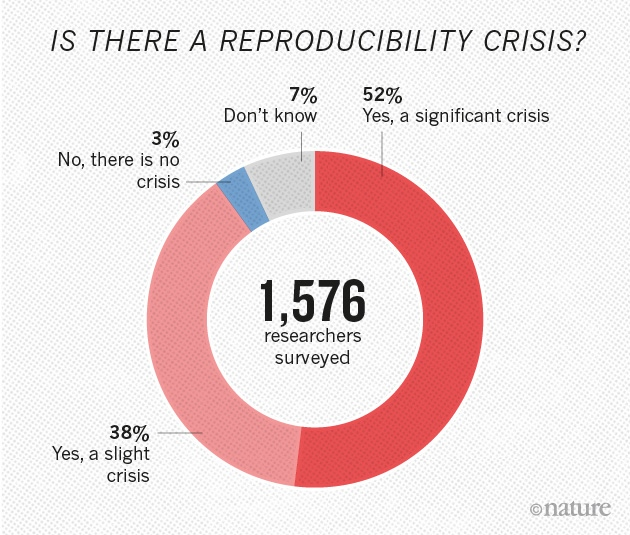
\includegraphics{reproducibility-graphic-online1.jpeg}\\

\section{The Survey}\label{the-survey}

\hfill\break
In the survey \footnote{The survey can be downloaded
  \href{Reproduciblility\%20Questionnaire.xml}{here}} respondents were
asked to rate 11 different approaches to improving reproducibility in
science . Below is the list order by the most highly rated:

\begin{itemize}
\tightlist
\item
  Better understanding of statistics
\item
  Better mentoring/supervision
\item
  More robust design
\item
  Better teaching
\item
  More within-lab validation
\item
  Incentives for better practice
\item
  Incentives for formal reproduction
\item
  More external-lab validation
\item
  More time for mentoring
\item
  Journals enforcing standards
\item
  More time checking notebooks
\end{itemize}

\end{document}
